\documentclass{article}
\usepackage[utf8]{inputenc}
\usepackage{graphicx}
\usepackage{listings}
\usepackage{color}

\definecolor{dkgreen}{rgb}{0,0.6,0}
\definecolor{gray}{rgb}{0.5,0.5,0.5}
\definecolor{mauve}{rgb}{0.58,0,0.82}

\lstset{frame=tb,
  language=C,
  aboveskip=3mm,
  belowskip=3mm,
  showstringspaces=false,
  columns=flexible,
  basicstyle={\small\ttfamily},
  numbers=none,
  numberstyle=\tiny\color{gray},
  keywordstyle=\color{blue},
  commentstyle=\color{dkgreen},
  stringstyle=\color{mauve},
  breaklines=true,
  breakatwhitespace=true,
  tabsize=3
}
\title{Distributed System - Lab 2}

\begin{document}

\maketitle

\section{RPC service design}
    This RPC server provides 3 services for client:
    \begin{itemize}
        \item Upload a file to server
        \item Download a file from server
        \item List out files stored in server
    \end{itemize}
    \begin{figure}[h]
        \centering
        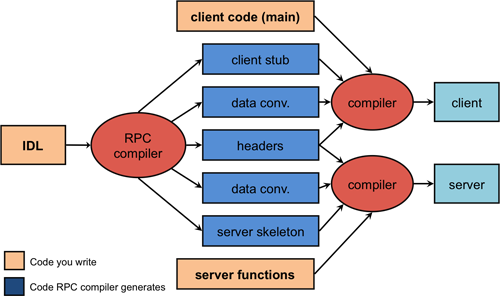
\includegraphics[width=\textwidth,height=200px]{image/rpc-compilation.png}
        \caption{RPC compilation}
        \label{fig:my_label}
    \end{figure}

In order to design the RPC service, first I have create the IDl then use rpcgen to generate template code. Next, I create function in both client and server to handle above three services.
\newpage
    \begin{figure}[h]
        \centering
        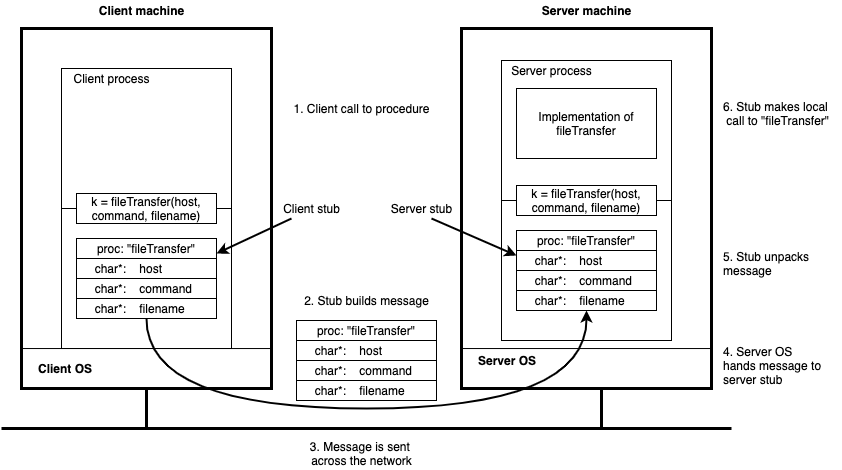
\includegraphics[width=1.2\textwidth]{image/RPCservice.png}
        \caption{RPC service design}
        \label{fig:my_label}
    \end{figure}
The RPC service now look like Figure 2. Client sends a message to the server which include three parameters:
\begin{itemize}
    \item host: Host of the server.
    \item command: A string input from command line specify the service that client want to use (upload/download/getdir).
    \item filename: Name of the file client request to upload/download.
\end{itemize}

\section{System organization}
The system is organized basically as client-server because there is only communication between client and server. This organization have not support file transfering between client and client
    \begin{figure}[h]
        \centering
        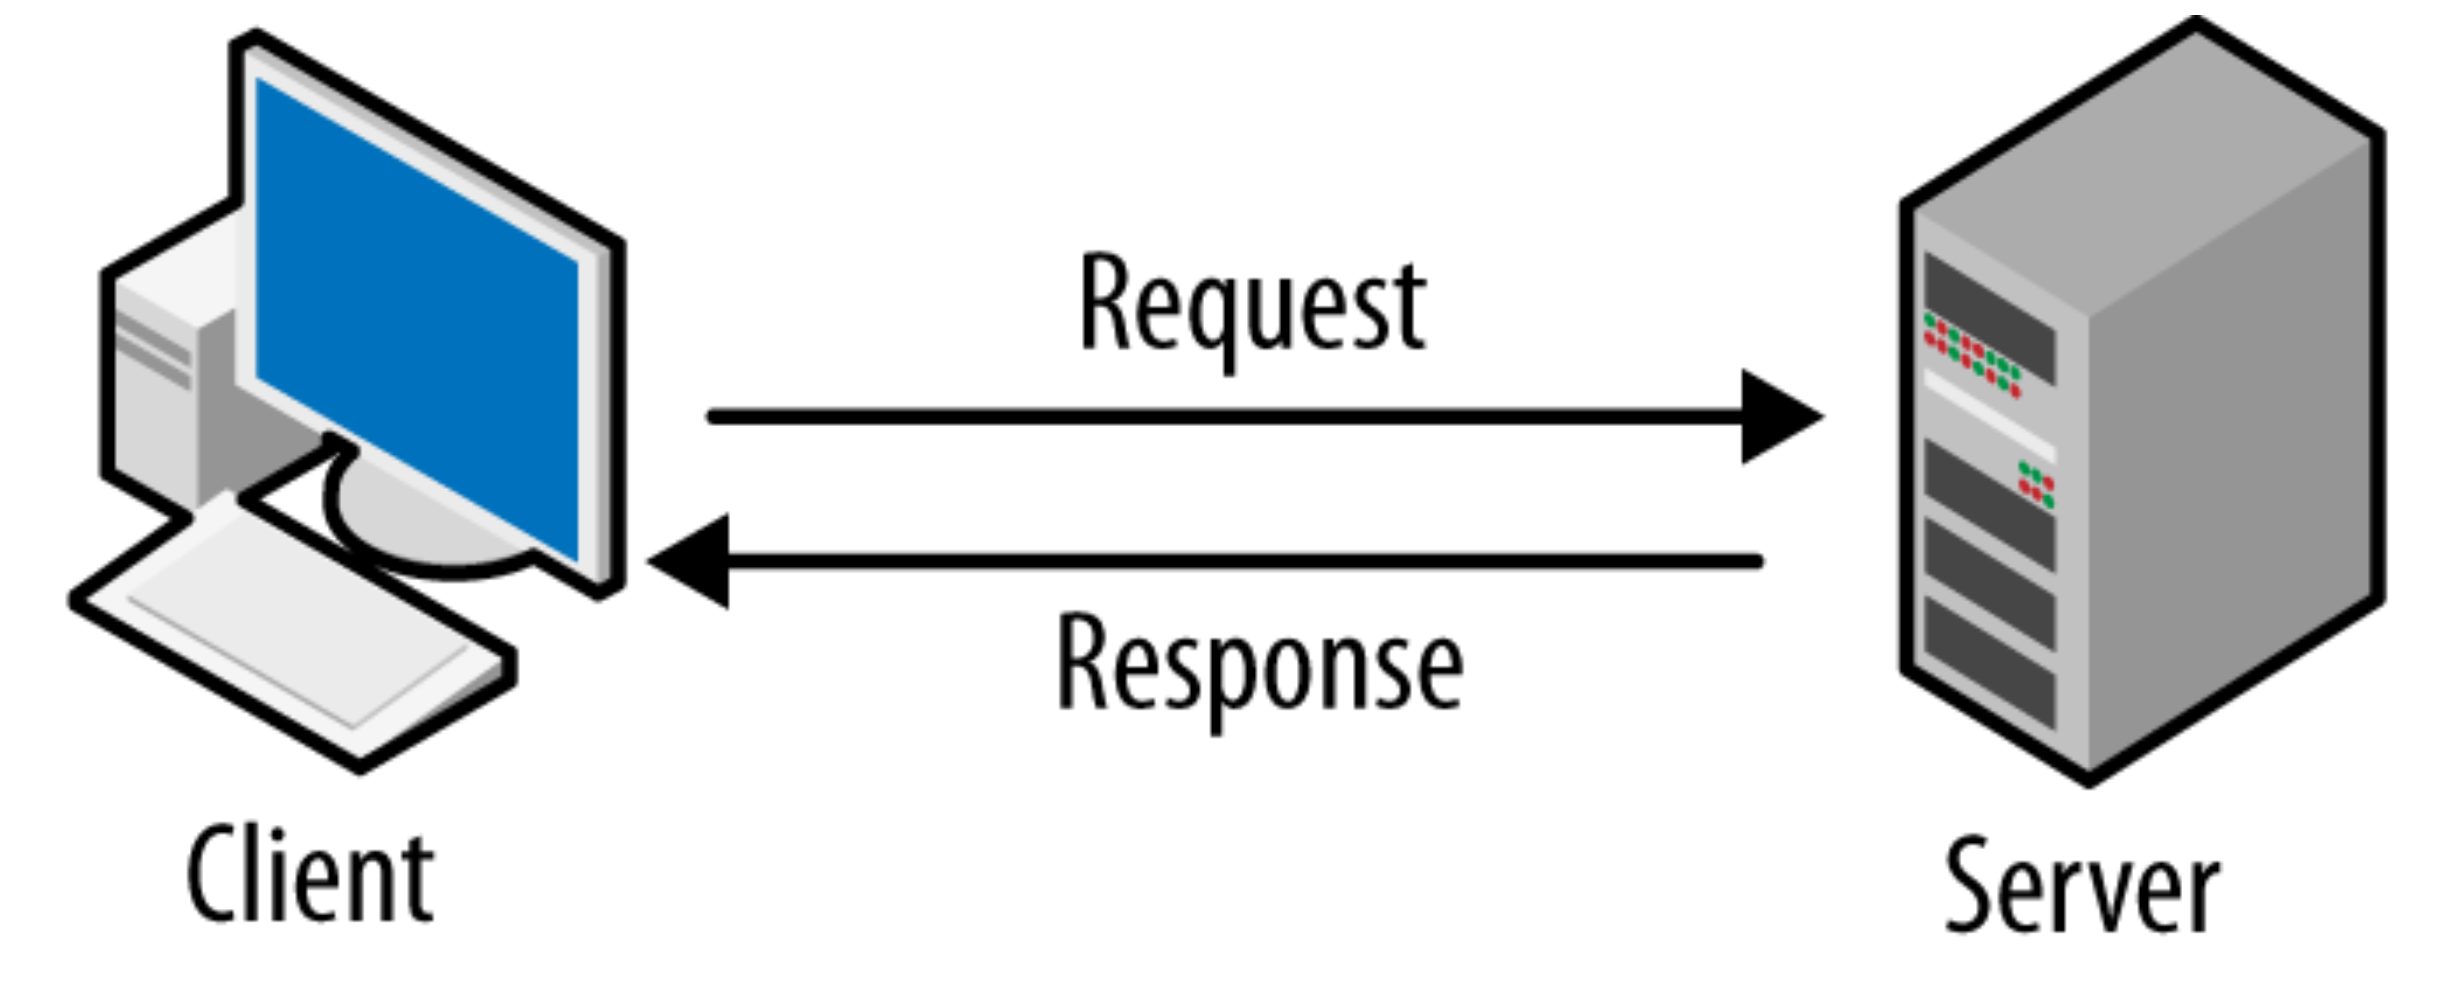
\includegraphics[width=0.5\textwidth,height=60px]{image/client-server-1.png}
        \caption{System organization}
        \label{fig:my_label}
    \end{figure}
\newpage
\section{Implementation}
First thing is starting the server. In window run:
\begin{lstlisting}
./file_transfer_server
\end{lstlisting}
In Mac OS, I need to be root to start the server:
\begin{lstlisting}
sudo ./file_transfer_server
\end{lstlisting}

\subsection{Upload}
Code snippet for server side:
\begin{lstlisting}
    if(argp->flag == 1){//get the data, dump it to a file
		FILE *fp;
		char *filename = argp->dirname;
		char prefix[10] = "uploaded_";
		strcat(prefix,filename);
		fp = fopen(prefix, "ab+");
		if(fp==NULL)
		{
		printf("Sorry the file cannot be opened");
		exit (1);
		}
		//printf("%s",argp->sendBuff);
		fwrite(argp->sendBuff, 1,strlen(argp->sendBuff),fp);
		fclose(fp);
	}
\end{lstlisting}
For client side, to upload a file to the server
\begin{lstlisting}
./file_transfer_server localhost -upload filename
\end{lstlisting}
Code snippet for client side:
\begin{lstlisting}
    if(strcmp(command,"-upload") == 0){
		ft_1_arg.flag = 1;
		fp = fopen(filepath,"rb");
		char *actual_file = get_file_name_from_path(filepath, "/");
		if(fp==NULL){
			printf("Sorry the file cannot be opened");
			exit (1);
		}
		strcpy(ft_1_arg.dirname, actual_file);
		while(1){
			memset(&(ft_1_arg.sendBuff[0]), 0, sizeof(ft_1_arg.sendBuff)); //clear the whole buffer before sending anything
			int nread = fread(ft_1_arg.sendBuff,1,1025,fp); //read from the file
			if(nread > 0){//if you read successfully then send this data
			result_1 = ft_1(&ft_1_arg, clnt);
			}
			if (nread < 1025){
				if(ferror(fp)) printf("Error reading\n");
			break;
			}
		}
		//finally close the file
		fclose(fp);
\end{lstlisting}

\subsection{Download}
Code snippet for server side:
\begin{lstlisting}
    else if(argp->flag == 2){// get a request to send the file
		FILE *fp;
		fp = fopen(argp->dirname, "rb+");
		if(fp==NULL)
		{
		printf("Sorry the file cannot be opened");
		exit (1);
		}
		memset(&(argp->sendBuff[0]), 0, sizeof(argp->sendBuff)); //clear the whole buffer before sending anything
		int nread = fread(argp->sendBuff,1,1025,fp); //read from the file
		result = *argp;
		if(nread > 0 && nread == 1025){//if you read successfully then send this data
		return &result;
		}else if(ferror(fp)){
		printf("Error reading\n");
		}else{
		result.flag = 4;
		return &result;
		}
		//finally close the file
		fclose(fp);
	}
\end{lstlisting}
For client side, to upload a file to the server
\begin{lstlisting}
./file_transfer_server localhost -download filename
\end{lstlisting}
Code snippet for client side:
\begin{lstlisting}
    else if(strcmp(command,"-download") == 0){
		ft_1_arg.flag = 2;
		strcpy(ft_1_arg.dirname, filepath);
		char *actual_file = get_file_name_from_path(filepath, "/");
		FILE *fp;
		fp = fopen(actual_file, "ab+");
		if(fp==NULL){
			printf("Sorry the file cannot be opened");
			exit (1);
		}
		do{
			result_1 = ft_1(&ft_1_arg, clnt);
			//printf("%s", result_1->sendBuff);
			fwrite(result_1->sendBuff, 1,strlen(result_1->sendBuff),fp);
		}while(result_1->flag!=4);
		}
\end{lstlisting}

\subsection{Get Directory}
Code snippet for server side:
\begin{lstlisting}
    DIR *dp;
		struct dirent *ep;
		dp = opendir ("./");
		if (dp != NULL)
		{
		while (ep = readdir (dp)){
		char fname[50];
		memset(&(fname[0]), 0, sizeof(fname));
		strcpy(fname, ep->d_name);
		strcat(fname, "—");
		strcat(result.dirname, fname);
		}
		}else
		perror ("Couldn’t open the directory");
		}
		return &result;
\end{lstlisting}
For client side, to upload a file to the server
\begin{lstlisting}
./file_transfer_server localhost -getdir
\end{lstlisting}
Code snippet for client side:
\begin{lstlisting}
    else if(strcmp(command,"-getdir") == 0){
			result_1 = ft_1(&ft_1_arg, clnt);
			//puts(result_1->dirname);
			char *token = strtok(result_1->dirname,"—");
			while( token != NULL ){
				printf( " %s\n", token );
				token = strtok(NULL, "—");
			}
		}
\end{lstlisting}

\section{Contribution}
    Nguyen Le Thanh Ha - BI9-094
\end{document}
